% subsection title
\section*{Clustering. Which players are similar? (15 points)}
%\addcontentsline{toc}{section}{Clustering. Which players are similar? (15 points)}
\label{subsec:3Q1}

\paragraph{Introduction}Using the \texttt{stats} library in R, the purpose of this part is to determine the 'closest' players thanks to the kmeans algorithm. We should not forget the main idea of the NBA analysis started in the assignment 1: \textit{explain the factors that influence the player's salary}. After defining 'closest', we will explain the approach used in order to conduct the analysis.

In the context of NBA players, two players are close if their statistics (\texttt{weight}, \texttt{height}, \texttt{age}, \texttt{experience} and its games statistics) are similar. We aim to cluster the current NBA active players in order to understand the characteristics of the differents groups and how it influence their salary.

\paragraph{Data}The first step to conduct the analysis is to build the dataset. To do that, we used the data scraped during the assignment 1 as follows:

\begin{itemize}
\item Filtering
	\begin{enumerate}
	\item extract the profile of the active players into the \texttt{active\_player\_profile} dataframe (attributes: \texttt{PlayerID}, \texttt{name}, \texttt{shoots}, \texttt{weight}, \texttt{height}, \texttt{dob}, \\ \texttt{birth\_city}, \texttt{birth\_state}, \texttt{experience} and \texttt{age})
	\item extract the most recent salary recorded for the active players into the \texttt{active\_salaries} dataframe (attributes: \texttt{PlayerID}, \texttt{Season}, \texttt{Team},\\ \texttt{FranchiseID} and \texttt{Salary})
	\item extract the totals statistics for the current active players into the \\ \texttt{active\_totals\_final} dataframe (attributes: \texttt{PlayerID}, \texttt{Season}, \texttt{Age},\\ \texttt{FranchiseID}, \texttt{Lg}, \texttt{Pos}, \texttt{G}, \texttt{GS}, \texttt{MP}, \texttt{FG}, \texttt{FGA}, \texttt{FG\%}, \texttt{X3P}, \texttt{X3PA}, \texttt{X3P\%}, \texttt{X2P}, \texttt{X2PA}, \texttt{X2P\%}, \texttt{eFG\%}, \texttt{FT}, \texttt{FTA}, \texttt{FT\%}, \texttt{ORB}, \texttt{DRB}, \texttt{TRB}, \texttt{AST}, \texttt{STL}, \texttt{BLK}, \texttt{TOV}, \texttt{PF} and \texttt{PTS})
	\end{enumerate}
\item Merging
	\begin{enumerate}
	\item merge \texttt{active\_player\_profile} with \texttt{active\_salaries} into the \\ \texttt{player\_information\_inter} dataframe
	\item merge \texttt{player\_information\_inter} with \texttt{active\_totals\_final} into the \texttt{player\_information} dataframe
	\end{enumerate}
\end{itemize}

The \texttt{player\_information} dataframe contains 600 active players but at the end the kmeans algorithm is applied to only 531 active players. Indeed, the dataset is build so that for each active player we keep its last salary recorded - note that the salary of the current season can be missing - with its corresponding totals statistics for the same team and season - some players change team during the season and so have two records in salaries and teams for the same season.

\paragraph{Attributes chosen to explain the player's salary}The salary is influenced directly by the \texttt{experience} of the player and by all the statistical attributes that gather data about the player's performance (see \texttt{active\_totals\_final} for the list).

\paragraph{kmeans algorithm}The main issue in dealing with the kmeans algorithm is the difficulty in finding the optimal number of centrois (\texttt{k}). In order to find the better parameter we use the cluster-diameter mean analysis. The figure below show the result for our dataset. 

\begin{figure}[h!]
\centering
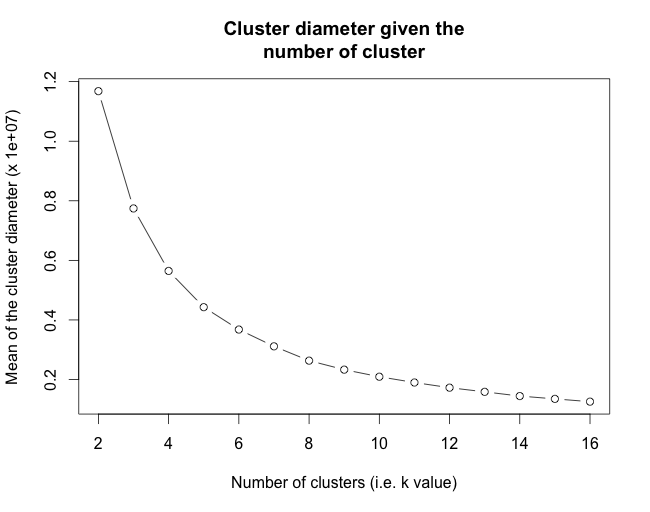
\includegraphics[width=0.75\textwidth]{images/diameter_kmeans}
\end{figure}

\paragraph{}From that figure we cannot get directly the optimal \texttt{k} without being sure of the chosen \texttt{k}. Then, we proceed to a deeper analysis. The idea is to compute the divergence of the slope from the \texttt{k}\ts{th} to the \texttt{k+1}\ts{th} clusters. The table below shows the results computed.\\

\begin{tabular}{|l|l|l|l|l|l|}
\hline \texttt{k} & \texttt{diameter} & \texttt{slope} & \texttt{variation} (\%) & \texttt{divergence} (\%) & \texttt{diff\_div} (\%) \\ 
\hline 2 & 11680914 & 0.00 & 0.000000 & 0.00000 & 0.00000000 \\ 
\hline 3 & 7742893 & -3938021.36 & -Inf & 0.00000 & 0.00000000 \\ 
\hline 4 & 5644795 & -2098098.18 & 46.722021 & 46.72202 & 46.72202131 \\ 
\hline 5 & 4429310 & -1215484.24 & 42.067333 & 69.13465 & 22.41262459 \\ 
\hline 6 & 3677566 & -751744.45 & 38.152678 & 80.91061 & 11.77595914 \\ 
\hline 7 & 3113996 & -563570.26 & 25.031670 & 85.68900 & 4.77839436 \\ 
\hline 8 & 2633222 & -480773.84 & 14.691410 & 87.79149 & 2.10248776 \\ 
\hline 9 & 2330790 & -302431.24 & 37.094905 & 92.32022 & 4.52873621 \\ 
\hline 10 & 2093675 & -237115.06 & 21.597036 & 93.97883 & 1.65860413 \\ 
\hline 11 & 1899240 & -194435.25 & 17.999620 & 95.06262 & 1.08378818 \\ 
%\hline 12 & 1725969 & -173271.03 & 10.884968 & 95.60005 & 0.53743270 \\ 
%\hline 13 & 1586060 & -139909.44 & 19.253993 &  96.44721& 0.84716638 \\ 
\hline 
\end{tabular} 

\paragraph{}The \texttt{variation} is the \% of variation between the \texttt{k}\ts{th} and the \texttt{k-1}\ts{th} slopes. The \texttt{divergence} is the variance of each slope from the first one ($k=3$). Finally, the \texttt{diff\_div} is the variation between the \texttt{k}\ts{th} and the \texttt{k-1}\ts{th} of the \texttt{divergence}.

\paragraph{}Theses numbers conduct us to choose $k=6$. Indeed, for that value, the slope is up to $81\%$ different from the first slope. For $k=7$, the difference is of $85.7\%$. Thus, the variance of the \texttt{divergence} start becoming insignificant (about $4.7\%$ compare to previous which are about $>12\%$).

\paragraph{Cluster centroids}With $k=6$ and the previous attributes chosen, the kmeans algorithm output the same centers (it is 'stable'). The data below shows the difference from the mean.

\begin{minted}[frame=single,linenos,mathescape,fontsize=\small]{r}
> km_final$centers
       Salary     weight      height experience        age         G
1 -1796384.28 -0.3256596 -2.92232958  0.1824454 -0.1335164  1.199887
2 -3013671.09  0.1906397 -0.06971589 -1.9161103 -0.9032700 -7.110760
3  2944608.94  0.1305320 -1.79908192  2.2301966  1.5640596  8.234934  
4  7231951.43 -1.7428654  6.30508475  2.4661741  1.2319281  4.138780 
5 13826170.47  0.4130320  8.31841808  3.1420716  1.3221846  7.864934 
6    67988.91  0.5091240 -0.13169686  0.7296578  0.2513800  5.433210  
          GS         MP         FG         FGA        X3P       X3PA
1 -1.6590457  -17.75074  -8.767042   -17.67844  -2.952233  -5.719221
2 -7.9715261 -311.13325 -57.616928  -123.64942 -11.010633 -30.181503
3  8.1495115  367.00992  64.626942   142.05535  21.107639  54.038518
4 16.5513545  370.29958  75.619731   150.50847   0.991453   4.316964
5 24.8426365  643.31804 172.798192   359.58847  18.648889  51.924143
6  0.6371193  148.42425  18.100721    43.48549   8.750958  22.930580
         X2P      X2PA         FT        FTA         ORB          PF
1  -5.814809 -11.95922  -7.560660  -8.029586   0.0530475   0.9898798
2 -46.606295 -93.46792 -28.379378 -35.958352 -13.8642266 -22.2423341
3  43.519303  88.01683  30.527395  35.792844  10.9232286  23.7870468
4  74.628278 146.19151  36.672027  51.408228  25.2361292  23.0502680
5 154.149303 307.66433 119.181770 148.632844  32.4751036  32.0564218
6   9.349763  20.55491   4.330736   4.172154   4.5606208  15.1722839
         DRB        TRB       AST         STL      BLK       TOV        PTS
1  -4.401007  -4.347959  -3.01709  -0.8676804 -1.08407  -1.97136  -28.04698
2 -45.046135 -58.910361 -33.95444 -10.1036953 -5.92591 -19.98455 -154.62387
3  42.724723  53.647952  30.13609   9.9164901  4.22345  17.47066  180.88892
4  72.749964  97.986093  60.06678  14.7362017 15.70983  29.32362  188.90294
5 121.165348 153.640452 108.44422  21.9577401 14.18470  62.22003  483.42704
6  14.767647  19.328268   5.02169   5.1287746  1.34378   6.55704   49.28314

km_final$size
[1]  107  209  64  39  25  87
\end{minted}

\paragraph{Interpretation}By analyzing the centers coordinates, we can derive the caracteristics of the different player clusters. We can assume the clusters are as follows: \textbf{rookies} (cluster 2), \textbf{intermediate experienced} (cluster 1), \textbf{advanced experienced} (cluster 6), \textbf{seniors 2P} (cluster 4), \textbf{seniors 3P} (cluster 3) and \textbf{all-stars} (cluster 5). The experience is the attribute that influence the most the player salary. The more experienced a player is, the higher salary he earns - senior players are above $3$ millions. At the opposite, the rookies are under $3$ millions the mean salary. Note also that the age is strongly correlated with experience. The more experienced a player is, the higher the probability to be older and finally the higher salary he earns. Let's understand deeper the differences between clusters.

\subparagraph{Rookies - 209 players}Since rookies have played lesser games than other players, their statistics are lower - the centroid's coordinates are all below the mean. But be careful, that doesn't mean the players are bad. It just translates a lack of experience compared to experienced and seniors players. Players is this category can be very promising.

\subparagraph{Intermediate experienced - 109 players}This category corresponds to players with some experience in NBA (equals to the mean). This is by no doubt the category of the worst players since it concerns the players with experience but with statistics below the mean. One important thing is the \texttt{height} which is the lower - of $3cm$ from the mean - between the clusters. Since basket-ball uses to be a sport with tall players, we can induce that this attribute may influence the salary ($<1.7$ million). We should be aware of this result. Indeed, Tony Parker is a 'small' player but still earns more than $12.5$ million USD. This cluster groups the worst players (lower statistics).

\subparagraph{Advanced experienced - 87 players}This category group the players with some experience in NBA (a little higher than the mean) but who do not separate from the crowd. Their statistics shows they are close to the mean - including the salary.

\subparagraph{Seniors 2P and Seniors 3P - 39 and 64 players}These two categories are quite complementary. What distinguish the most these clusters are the difference in \texttt{height} of the players (about $8cm$) and the salary. That difference influence also their statistics. Indeed, seniors 2P have higher statistics in \texttt{X2P}, \texttt{X2PA}, \texttt{DRB} \texttt{TRB}, \texttt{AST}, \texttt{STL} and \texttt{TOV} than seniors 3P. Since seniors 2P are taller, we can assume they tend to be positionned under the basket, then are prone to score more $2$ points. In the opposite, seniors 3P, smaller, are prone to score more $3$ points and their position requires less defensive than seniors 2P.

\subparagraph{All-stars - 25 players}This last category contains the best players of the current NBA season. As expected, they have the higher statistics in all the attributes making them the most experienced and talented NBA players. They obviously are the best paid players ($13.8$ million above the mean).